\documentclass{article}
\usepackage{pythonhighlight}
\usepackage{graphicx}
\usepackage{ctex}
\usepackage[left=3cm,top=3cm,right=3cm]{geometry}
\usepackage{hyperref}
% TITLE PAGE CONTENT %%%%%%%%%%%%%%%%%%%%%%%%
%%%%%%%%%%%%%%%%%%%%%%%%%%%%%%%%%%%%%%%%%%%%%
\newcommand{\labno}{12}
\newcommand{\labtitle}{EE208 SIFT}
\newcommand{\authorname}{周李韬}
\newcommand{\studentno}{518030910407}
\newcommand{\classno}{F1803016}
% END TITLE PAGE CONTENT %%%%%%%%%%%%%%%%%%%%


\begin{document}

\begin{center}
{\LARGE \textsc{Laboratory No. \labno:} \\ \vspace{4pt}}
{\Large \textsc{\labtitle} \\ \vspace{4pt}} 
\rule[13pt]{\textwidth}{1pt} \\ \vspace{15pt}
{\large By: \authorname \\ \vspace{10pt}
No. \studentno \\ \vspace{10pt}
SJTU \classno \\ \vspace{10pt}
\today \vspace{20pt}}
\end{center}



\section{实验准备}

\subsection{实验环境}
\begin{itemize}
\item\textbf{Environment} Python 3.7
\item\textbf{Packages} numpy 1.15.4, opencv-python 3.4.3.18
\item\textbf{Tools} Pycharm 2018.2 on Windows 10
\end{itemize}

\subsection{实验目的}

本实验中,我们需要练习使用Opencv实现SIFT算法的图像匹配。

\subsection{实验原理}

SIFT算法是David Lowe于1999年提出的局部特征描述子,并于2004年进行了更深入的发展和完善。Sift特征匹配算法可以处理两幅图像之间发生平移、旋转、仿射变换情况下的匹配问题,具有很强的匹配能力。我们在本实验中将通过SIFT算法实现图像特征点的匹配与图像匹配度的计算。

SIFT算法的计算主要包含以下几个步骤:
\paragraph{尺度空间极值点提取} SIFT算法要求为图像建立多个尺度空间,模拟图像的缩放产生的差异,以避免不同尺度大小下角点、边点的错识别。本实验中将采用图像金字塔和Harris角点检测的手段替代这一实现起来较为复杂的算法。


\paragraph{计算关键点主方向} SIFT描述子之所以具有旋转不变的性质,是因为它实现了在图像坐标系和物体坐标系之间变换。SIFT描述子把以关键点为中心的邻域内的主要梯度方向作为物体坐标系的X方向,因为该坐标系是由关键点本身的性质定义的,因此具有旋转不变性。具体计算方法如下,对某关键点$I_{(x_0,y_0)}$,对于它$m\times m$邻域的每个点,计算其梯度、梯度方向,随后为梯度方向在每个以10度为单位的bins内投票,确定关键点的主方向(即投票最高的bins)。该方向即为物体该角点的物体坐标系方向。


\paragraph{SIFT描述子计算} SIFT描述子是一个在特征点周围16个的4*4的像素块中,每个块内按照求主方向的方式把360度分成8个bins,统计梯度方向直方图,生成8维的直方图向量叠加,每个关键点可生成4*4*8=128维的SIFT描述子。该描述子能够达到描述物体周围特征的目的。注意到该计算需要在特征点的物体坐标系下计算,因此要对坐标进行以下旋转变化。
$$\left(\begin{array}{l}{x^{\prime}} \\ {y^{\prime}}\end{array}\right)=\left(\begin{array}{cc}{\cos \theta} & {-\sin \theta} \\ {\sin \theta} & {\cos \theta}\end{array}\right)\left(\begin{array}{l}{x} \\ {y}\end{array}\right)$$

经过旋转变化后的点不一定位于像素点上,因此需要对像素点做插值计算,本实验中采用了双线性插值。

\paragraph{SIFT描述子匹配} 再开始匹配之前,我们需要对特征向量进行归一化处理,去除光照变化的影响。

$$
f=f_{0} \cdot \frac{1}{\left|f_{0}\right|}
$$

通过两个SIFT描述子做内积,我们就可以得到两个SIFT描述子的相似度,可表示为
$
s\left(f_{1}, f_{2}\right)=f_{1} \cdot f_{2}
$

\section{实验步骤}

\subsection{图像预处理}

图像预处理包括灰度化和求梯度值,预先将图片的梯度值计算完成有助于减少调用时的计算量,在本实验中,我们选择了Prewitt算子,并且将预处理的过程封装为SIFTimg类的构造函数,使程序结构更清晰。此外,我们调用了cv2.filter2D函数,使代码更简洁。Python脚本如下。
\begin{python}
class siftIMG:
    def __init__(self,src):
        img = cv2.imread(src, cv2.IMREAD_COLOR)
        img = cv2.cvtColor(img, cv2.COLOR_BGR2GRAY)
        self.orgimg = cv2.imread(src, cv2.IMREAD_COLOR)
        self.img = np.float32(img)                            # 读取图像,灰度化

        krn1 = np.array([[-1,0,1],[-1,0,1],[-1,0,1]],dtype=np.float32)
        krn2 = np.array([[-1, -1, -1], [0, 0, 0], [1, 1, 1]],dtype=np.float32)
        self.gx = cv2.filter2D(self.img, -1,krn2)
        self.gy = cv2.filter2D(self.img, -1, krn1)            # 计算x,y方向梯度

        self.height = img.shape[0]                            # 计算梯度幅值和角度
        self.width = img.shape[1]
        self.grad = np.zeros((self.height, self.width), float)
        self.theta = np.zeros((self.height, self.width), int)
        for x in range(1,self.height-1):
            for y in range(1,self.width-1):
                self.grad[x][y] = math.sqrt(gx[x][y] ** 2 + gy[x][y] ** 2)
                self.theta[x][y] = math.atan2(gy[x][y],gx[x][y])/math.pi * 180
\end{python}

\subsection{计算特征点主方向}

根据上文的原理简述,我们计算了特征点的主方向。在代码实现中,为了避免边缘处的下标越界错误,我们使用了一个try-except结构,认为图像边缘处的梯度为0,该结构本质上等同于在图片周围按相同的像素进行扩展。

\begin{python}
def calculate_main_dir(self,a,b,r):
    grads = list()
    for i in range(a-r,a+r+1):
        for j in range(b-r,b+r+1):
            try:
                grads.append((self.grad[i][j],self.theta[i][j]))
            except IndexError:
                grads.append((0,0))   # 处理图像边缘处下标越界的情况
    return self.vote_for_grad(grads)  # 返回一个关键点周围所有点的(梯度幅值,梯度角度)列表

def vote_for_grad(self,grads):
    voter = [0]*36
    for (g,t) in grads:
        voter[math.floor(t/10)] += g  # 统计关键点周围以幅值为权重的梯度角度立方图
    return 5+voter.index(max(voter))*10
\end{python}

\subsection{计算SIFT特征向量}

调用此前的计算特征点主方向函数,我们对图像坐标系内的邻域点进行坐标变化,我们同时写了get\_theta\_of、get\_grad\_of的插值函数,我们对各个像素块的像素点调用相关函数、访问此前计算的梯度结果,即可计算出特征点对应的SIFT特征向量。

\begin{python}
def SIFT_descripter(self, a, b):
    result = [0] * 128
    maindirr = ((self.height + self.width) // 80)
    t = self.calculate_main_dir(a, b, maindirr)
    blsize = 4
    for bx in range(blsize):
        for by in range(blsize):
            for i in range(blsize):
                for j in range(blsize):       # 遍历每一个像素块的每一个像素点
                    try:
                        x_r = (bx - 2) * 4 + i
                        y_r = (by - 2) * 4 + j
                        ltheta = self.get_theta_of(a + x_r * dcos(t) - y_r * dsin(t),
                                              b + x_r * dsin(t) + y_r * dcos(t))
                        result[(bx + by * blsize) * 8 + int(((ltheta + t) % 360) / 45)] += 1
                    except IndexError:         # 对溢出的边界点不作统计
                        pass
    return result
\end{python}

对图像中特征点的选取,我们采用了cv2中的goodFeaturesToTrack函数提取Harris角点。对这些角点遍历,调用上文的SIFT\_desrciptor函数,即可完成图像特征点的提取及SIFT向量的计算,Python代码如下。

\begin{python}
def get_cps_and_sifter(self,max_corner):
    self.extract_cps(max_corner)        # 提取最多max_corner个数的特征点
    sifters = list()
    for [[a, b]] in self.cps:
        tmp = np.array(self.SIFT_descripter(int(a), int(b)), dtype=float) # 调用SIFT特征向量计算函数
        norm = math.sqrt(np.inner(tmp, tmp))
        if norm != 0:
            tmp /= norm                 # 归一化处理
            sifters.append(((int(a), int(b)), tmp))
    return sifters                      # 返回结果,点的坐标和SIFT向量
\end{python}


\subsection{SIFT特征点匹配}

在这一段,我采用了两种方法。

首先,根据实验材料的提示,我们可以通过计算经过归一化后的两个特征向量内积,计算出两个SIFT特征点的相似度。相似度越接近1,就表明相似度越高。通过遍历提取计算结果中的最大值,我们即可达到SIFT匹配的效果,代码如下:
\begin{python}
def find_match(siftimg1,siftimg2,n):
    sifters1 = siftimg1.get_cps_and_sifter(n)
    sifters2 = siftimg2.get_cps_and_sifter(n)
    res = set()
    dists = list()
    for (k1, s1) in (sifters1):
        for (k2, s2) in (sifters2):
            dists.append((k1, k2, similarity(s1, s2)))
    print(dists)
    dist_sorted = sorted(dists, key=by_value)
    print(dist_sorted)  # 对结果按照similarity进行排序
    popedx = list()
    popedy = list()     # 用于记录已经被标记过的点,防止重复标记
    cnt = 0
    for (k1, k2, v) in dist_sorted:
        if (k1 not in popedx) and (k2 not in popedy):
            print(k1, k2, v)
            res.add((k1, k2))
            popedx.append(k1)
            popedy.append(k2)
            cnt += 1
        if v < 0.9 or cnt > 10:    # 设置阈值和退出条件
            break
    return res
\end{python}


但实验结果表明,该方法的缺点在于许多点尽管内积十分接近1,但存在很多不匹配的点,准确度较低,也不能达到较好的区分度。因此我采用了另一种方法,对similarity的计算,我们采用了两个SIFT特征向量的欧氏距离,此外,对图A中的每一个点,当我们寻找它在图B中的匹配点时,匹配的条件设为匹配度小于一定的阈值,且图B中第一匹配点与第二匹配点和A中待匹配点的匹配度之比要小于0.8,该方法可以更有效地去除那些由于特征不突出而产生的错配点,实现代码如下。

\begin{python}
def find_match2(siftimg1,siftimg2,n):
    sifters1 = siftimg1.get_cps_and_sifter(n)
    sifters2 = siftimg2.get_cps_and_sifter(n)
    res = set()
    for (k1, s1) in (sifters1):
        dists = list()   # 为图1中的待匹配点k1建立图2特征点的匹配度列表
        for (k2, s2) in (sifters2):
            dists.append((k1, k2, similarity(s1, s2)))
        one, second = find_min_and_second([i[2] for i in dists]) 
        # 对相似度列表进行遍历,找出最小值和第二最小值
        try:
            if (dists[one][2]/dists[second][2]) < 0.8:
                res.add((dists[one][0], dists[one][1]))
        except ZeroDivisionError:
            continue
    return res
\end{python}

在绘制匹配图像方面,我们调用了opencv中的drawMatches函数,注意在调用时,我们需要先将此前输出的结果封装成对应的KeyPoint、DMatch类供函数调用。
\begin{python}
res = find_match(img1,img2,n)
kp1 = [cv2.KeyPoint(x,y,1) for ((x,y),j) in res]
kp2 = [cv2.KeyPoint(x,y,1) for (i,(x,y)) in res]
matches = [cv2.DMatch(i,i,0) for i in range(len(res))]
result = cv2.drawMatches(img1.orgimg,kp1,img2.orgimg,kp2,matches,output)
cv2.imshow('img',result)
\end{python}



\subsection{基于SIFT特征的图片搜索与匹配}

在这一部分,我们采用内积的方法计算图片的匹配度,我们为每张图取50个特征点及对应的向量,进行n*n匹配,取匹配结果的最大的100个值相加,即记为两张图的匹配度。匹配度最大的图片即为程序认为匹配成功的图,对该图调用上文的函数进行对应特征点的绘图。

\begin{python}
match_rate = list()
img2 = siftIMG("./target.jpg")
for i in range(1,6):                   # 匹配图片
    data = "./dataset/"+str(i)+".jpg"
    img1 = siftIMG(data)
    res = find_match_rate(img1, img2, 50)
    match_rate.append(res)
    print (str(i)+" match rate: " + str(res))

maxidx = match_rate.index(max(match_rate))  # 得到匹配最大值图片
img1 = siftIMG("./dataset/"+str(maxidx+1)+".jpg")
output = np.zeros((400,400), np.uint8)
n = 50
res = find_match(img1,img2,n)               # 计算最佳匹配点进行绘图
...
cv2.imshow('img',result)
cv2.waitKey()
\end{python}


\section{实验结果}

对实验材料中的原图片和经过旋转和缩放的target图片进行特征点匹配,可以看到特征点的匹配未能达到理想的匹配效果,这是由于我们的算法中采用了较多的近似产生的。经过反复调试,取得了较为理想的三张实验结果如图\ref{fig1},\ref{fig2},\ref{fig3}所示。

\begin{figure}[htbp]
\centering
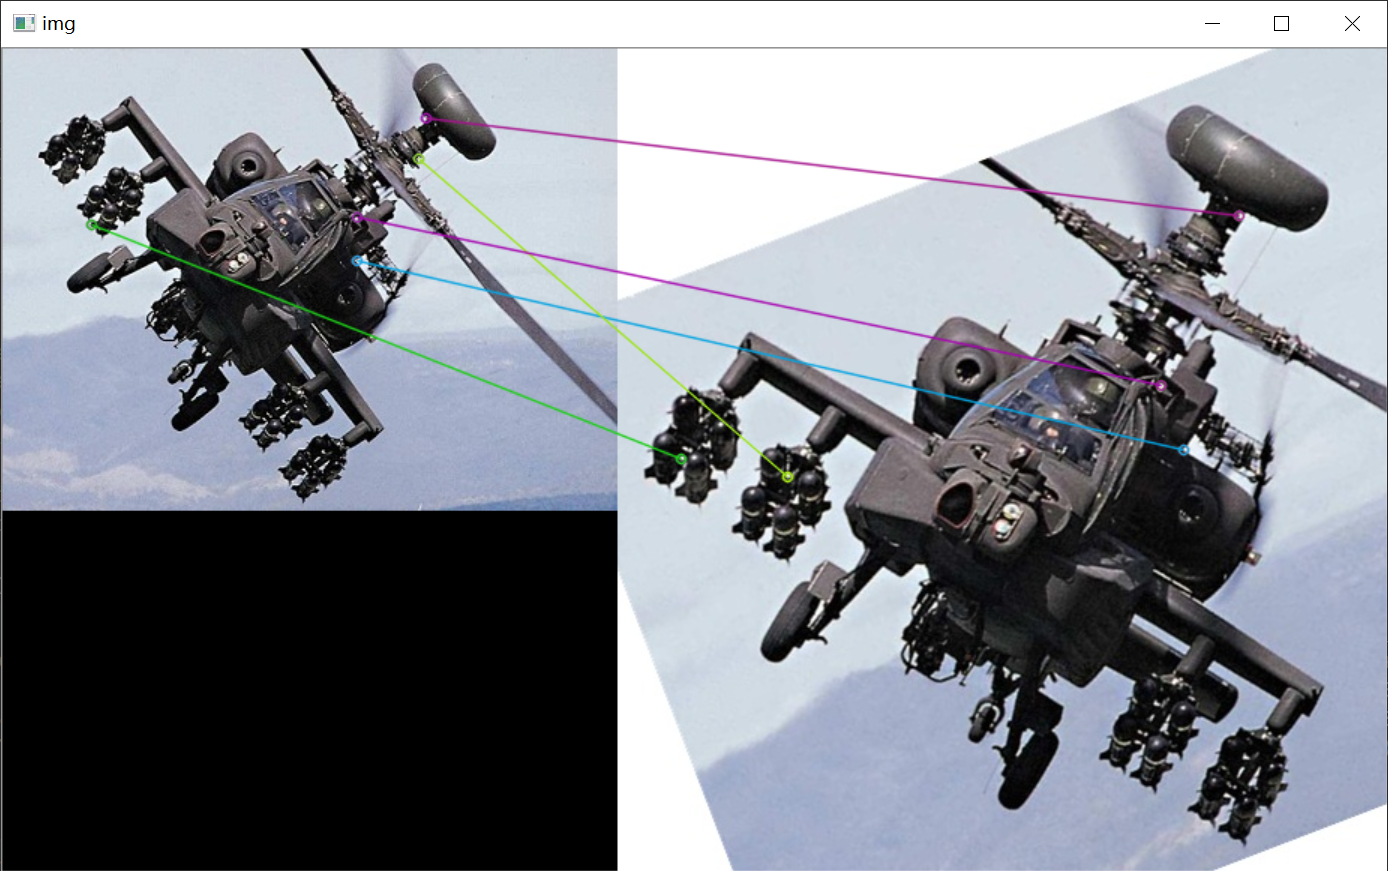
\includegraphics[width=13.5cm]{img/2.png}
\caption{特征点:5个,高斯模糊半径:3,阈值:0.85的匹配结果}
\label{fig1}
\end{figure}

\begin{figure}[htbp]
\centering
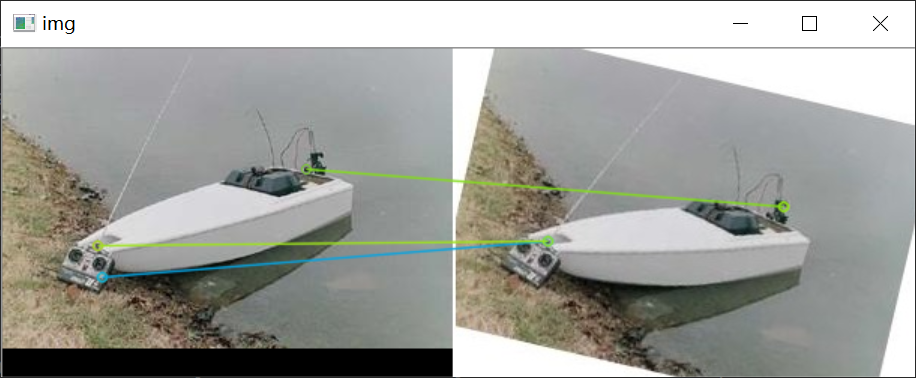
\includegraphics[width=13.5cm]{img/1.png}
\caption{特征点:5个,高斯模糊半径:3,阈值:0.9的匹配结果}
\label{fig2}
\end{figure}

\begin{figure}[htbp]
\centering
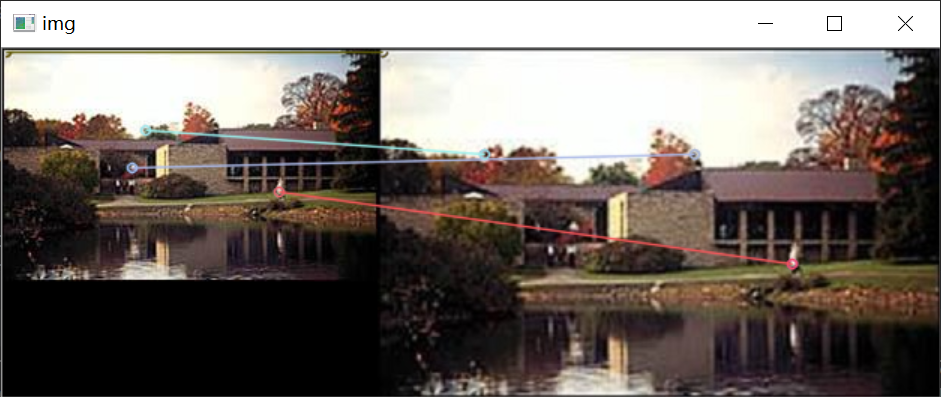
\includegraphics[width=13.5cm]{img/3.png}
\caption{特征点:10个,高斯模糊半径:3,阈值:0.85的匹配结果}
\label{fig3}
\end{figure}

运行图片匹配函数,我们得到的结果如图\ref{fig4}所示,程序成功识别了与原图匹配的图像,并作出了匹配点对应图。
\begin{figure}[htbp]
\centering
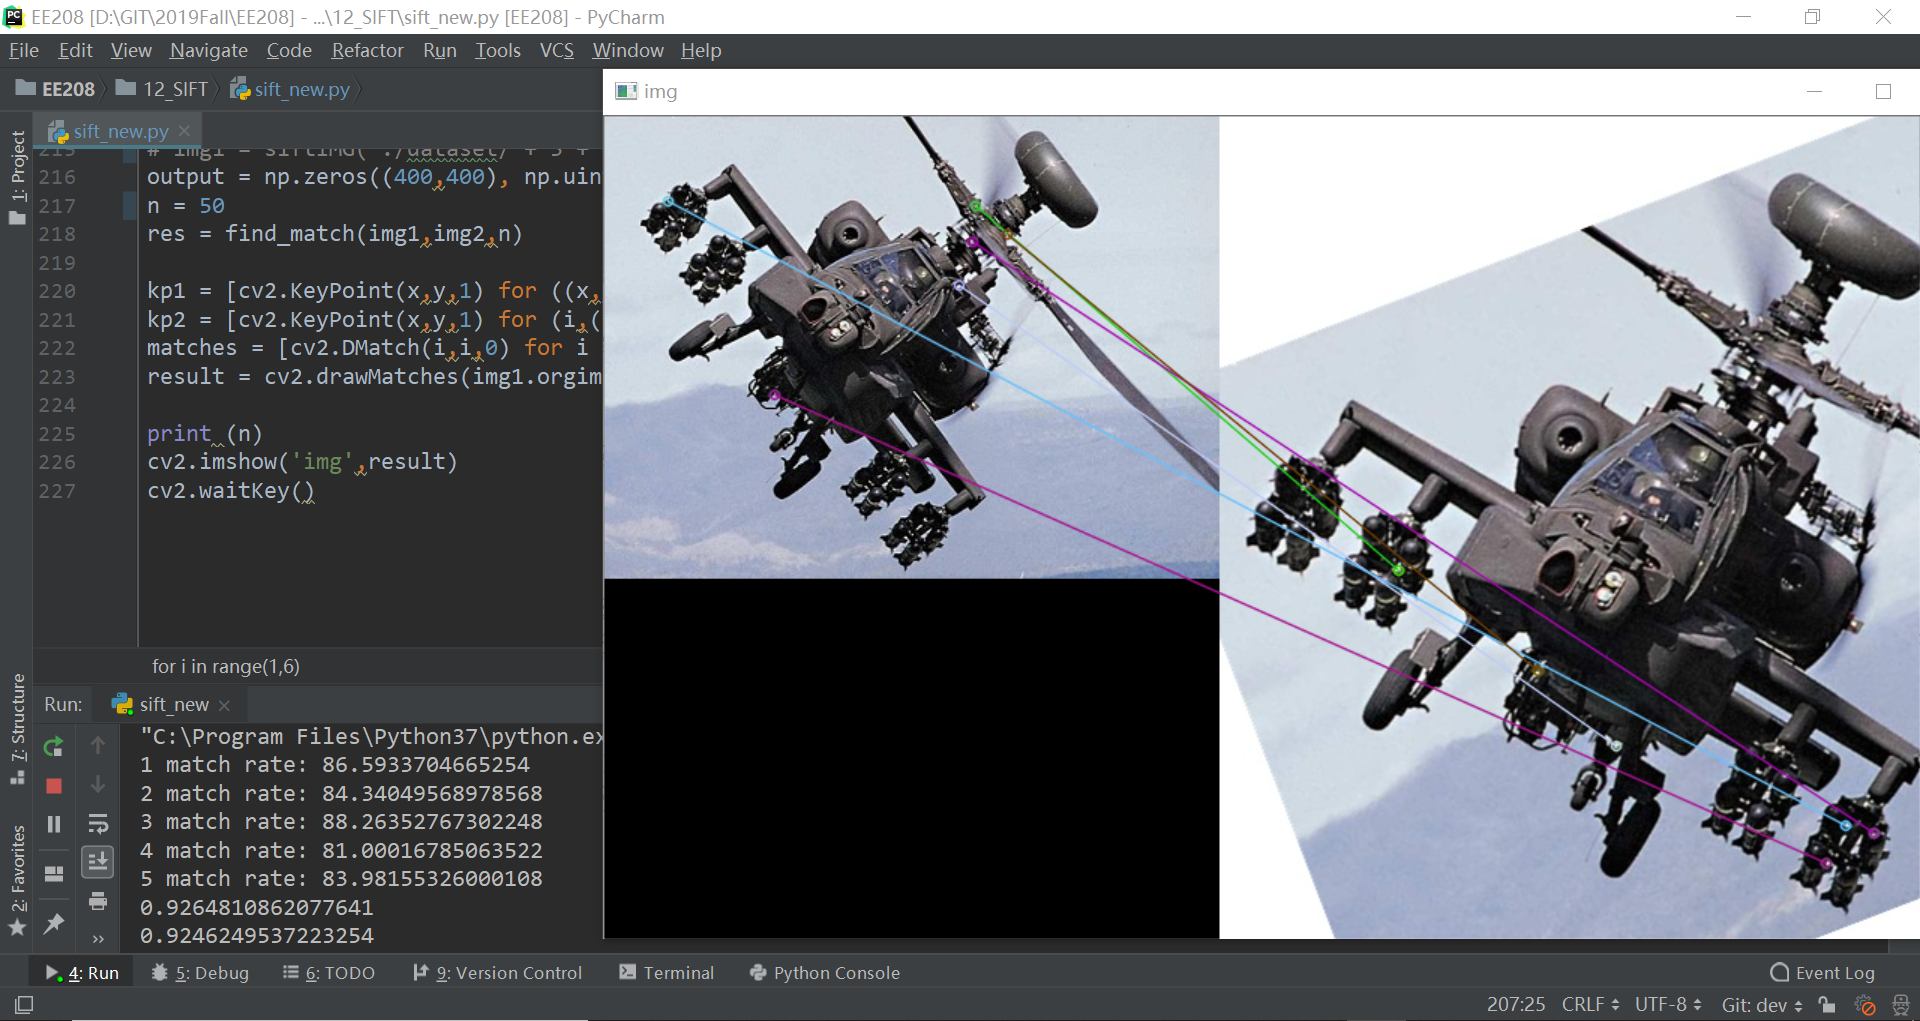
\includegraphics[width=13.5cm]{img/4.png}
\caption{SIFT匹配实例}
\label{fig4}
\end{figure}

\section{实验总结}
\paragraph{概述}
本实验中,我们通过OpenCV实现了图像边缘检测的SIFT算法特征点的匹配与图像匹配度的计算。

\paragraph{感想}
通过本次实验的学习,我通过手动实现SIFT算法的图像预处理、梯度计算、特征点提取、特征向量计算等过程,对图像处理中的特征提取方法和思想有了更深的理解,也掌握了更多OpenCV和numpy矩阵操作的技巧。

\paragraph{问题}
本次实验中遇到的问题为匹配度不高。由于实验方法本身的精度限制,如我们在提取Harris角点时没有进行尺度空间的差分,从而难以得到真正意义上准确的特征角点,如我们在计算梯度时采用的是微分算子,没有达到SIFT要求的精确度,因此即便经过反复修改代码和调试参数后,我们也没有得到显著可观的匹配度提高。但我依然在调试的过程中,对SIFT算法的思想和原理有了更深的认识。

\paragraph{创新}
本实验中采用了Prewitt算子计算梯度,相较材料中给出的梯度计算方法有一定的提升。此外,代码中也灵活运用了filter2D、math.atan2等函数,简化了代码,提高了可读性。本实验还将SIFT计算封装为一个类对象,提高了可用性。

\end{document}

